\section{Theory and literature}

Relevant theory will be: 
We envision using economic theories such as market equilibrium, Pareto efficiency and consumer choice theory. 
Statistical theory, such as the presumptions for regression to evaluate whether our data sources meet the requirements, and our model is robust. 
Neural networks, especially LSTM compared to other predictive models 

\subsection{Tensor flow}
Tensor flow is an open source library for numerical computation that makes machine learning and developing neural networks faster and easier (https://www.infoworld.com/article/3278008/what-is-tensorflow-the-machine-learning-library-explained.html).
It works by allowing the user to define a graph of computations that are then executed by the library. The graph is defined by the user by creating nodes that represent mathematical operations, and edges that represent the multidimensional data arrays (tensors) communicated between them. 
The library then optimizes the graph for execution on a CPU or GPU. 

\subsection{ARIMA --- SARIMAX}\label{ARIMATheory}

The ARIMA-model is one of the more popular and useful approaches to time series forecasting. The name is an acronym that stands for AutoRegressive Integrated Moving Average and the model utilizes these in order to predict future values solely on earlier values, it is therefore an univariate model. In order for the model to be able to predict, the data has to be stationary, which means that the mean, variance and covariance are constant over time. Time-series data is especially prone to be non-stationary, which can be solved either by log-transforming the data, convert it to a percentage change or by differencing which is further explained in~\ref{IntegratedTheory}.

The SARIMAX-model is an extension of the ARIMA-model that also takes external factors and seasonality into account in order to better predict future values. SARIMAX can therefore be a multivariate model. \parencite{hyndman_athanasopoulos_2021}

\subsubsection{Auto Regressive (AR)}\label{AutoRegressiveTheory}
The first part of the ARIMA acronym is the Auto Regressive part. Auto comes from the greek word autos and mean self, in this context it means that the model is regressing on itself. This part of the model can be written as follows:
\begin{equation}
y_{t} = c + \phi_{1}y_{t-1} + \phi_{2}y_{t-2} + \cdots + \phi_{p}y_{t-p} + \varepsilon_{t}
\end{equation}

Where c is a constant, $p$ is the number of lag observations or autoregressive terms, $\phi$ are the AR coefficients and $\varepsilon_{t}$ is the error term. $y_{t}$ is the data on which the AR-model is applied on. (\cite{oracle_ARIMA}) This model is a ``pure'' AR-model and relies therefore solely on its own lags. If $p$ is set to 1, the model looks at the previous value and tries to predict the next value. If $p$ is set to 2, the model looks at the previous two values and tries to predict the next value, and so on. (\cite{artley_2022})


\subsubsection{Integrated (I)}\label{IntegratedTheory}
The second part of the ARIMA acronym is the Integrated part. This part of the model is used to make the time series stationary. In the ARIMA-equation it is represented by the letter $d$ and is the number of differencing required to make the time series stationary. Usually the optimal amount of differencing is the least amount needed to make the data fluctuate around a well defined mean. (\cite{nau_2019}) It is the only form of converting the data to a stationary form that the ARIMA-model itself can do. Log-transforming and converting to a percentage change can only be done before the model is applied on the data. 

\subsubsection{Moving Average (MA)}\label{MovingAverageTheory}
The third and last part of the ARIMA acronym is the Moving Average part. This incorporates the dependency of an observation on the residual errors from a moving average model applied to lagged observations. \parencite{hayes_2019} This part of the model can be written as follows:
\begin{equation}
\hat{y} = c + \theta_1\epsilon_{t-1} + \theta_2\epsilon_{t-2} + \cdots + \theta_q\epsilon_{t-q}
\end{equation}

Where c is a constant, $q$ is the order of the moving average, i.e the number of lagged forecast errors. $\theta$ are the MA coefficients and $\varepsilon_{t}$ is the error term. For example, if $q$ is 1, the output relies solely on the errors from the previous time step. If $q$ is 2, the output relies on the errors from the previous two time steps. (\cite{hyndman_athanasopoulos_2021}) 

Combining these three parts of the ARIMA-model, we get the following general forecasting equation:
\begin{equation}
\hat{y}_t = c + \phi_1y_{t-1} + \phi_2y_{t-2} + \cdots + \phi_py_{t-p} + \theta_1\epsilon_{t-1} + \theta_2\epsilon_{t-2} + \cdots + \theta_q\epsilon_{t-q} + \epsilon_t
\end{equation}

\subsubsection{Seasonality (S)}\label{SeasonalityTheory}
For time-series data there can often incur a seasonal trend which is a pattern that repeats itself over a period of time. For example pollution levels in a city that might increase in the winter and decrease in the summer. This trend can be accounted for by adding a seasonal component to the model and where the ARIMA-model is written as ARIMA$(p,d,q)$, the SARIMA-model is written as SARIMA$(p,d,q) \times (P,D,Q)s$. Uppercase P, D and Q corresponds to the lowercase p, d and q, namely the AR, I and MA terms, but for the seasonal component. The $s$ is the number of periods in a season, for example if the data is measured daily, $s$ would be 7 if the seasonal trend is weekly.~\parencite{chang_et_al_2012}

\subsubsection{Exogenous variables (X)}\label{ExogenousTheory}
In addition to adding seasonality to the ARIMA model, one can also include exogenous variables and turn it into a multivariate model. This is often used when there is a clear correlation between the exogenous variable and the time series. For example, if the ARIMA model is used to predict the price of electricity, one could include weather data as one or several exogenous variables.~\parencite{elamin_fukushige_2018}


\subsection{Exploratory analysis}
Exploratory data analysis (EDA) is a method used to analyse datasets and summarize the main characteristics. It helps determine how best to manipulate datasources to get the answers needed. This makes it easier to discover patterns, anomalies, test hypotheses or checking assumptions (https://www.youtube.com/watch?v=QiqZliDXCCg). 

There are 4 steps involved in an exploratory data analysis: data collection, data cleaning, univariate analysis and bivariate analysis. 
Data collection simply consists of gathering the data needed for the analysis. 
Data cleaning is the process of removing or replacing missing values, outliers and other anomalies. Anamolies can disproportionally skew the data and hence adversely affect the results (https://www.simplilearn.com/tutorials/data-analytics-tutorial/exploratory-data-analysis).
Univariate analysis is analysis the data of only one variable. This is usually done by creating a histogram, boxplot or a frequency table.  
Bivariate analysis uses the data of two variables and compares them to each other. This establishes the correlation (or lack of) between the two variables. This is usually done by creating a correlation matrix or by plotting the data in a scatterplot. 

\subsection{Regression}
Regression analysis is a reliable method of identifying which variables have impact on a topic of interest. Regression analysis consists of two types of variables; dependent and independent. The dependent variable is the main variable or factor that aasdasd is trying to predict or understand. The independent variables are the factors that dasdasd hypothesize to have an impact on the chosen dependent variable. 

Linear regression models often use a "least-squares approach" to determine a line of best fit (regression line) to a given dataset. This line is the yellow line in the figure below. A square is the squared distance between a datapoint and the regression line. These values needs to be squared in order to not counteract each other.   

BILDE

When the process above has been completed a regression model is constructed. The genereal form of a \textbf{multiple linear regression model} is:  

- Regression, https://www.alchemer.com/resources/blog/regression-analysis/\\ 

https://www.investopedia.com/terms/r/regression.asp

\subsection{Neural networks}
\subsubsection{Recurrent Neural Network}
A recurrent neural network (RNN) is a special type of artificial neural network adapted for work with time series data or data that involves sequences (https://machinelearningmastery.com/an-introduction-to-recurrent-neural-networks-and-the-math-that-powers-them/). 
By adding a "feedback loop" RNNs are able to step through sequential input data while persisting the state of nodes in the hidden layer between steps. This is called "working memory". The hidden node concatenates its current input and the working memory from the previous steps, before the result is passed on to an activation function. The output from the activation function is then sent onwards to both the output layer, and forwarded on to the next iteration of the RNN (as the working memory)  (https://www.bouvet.no/bouvet-deler/explaining-recurrent-neural-networks).


BILDE
\subsubsection{Long Short-Term Memory} 
Long Short-Term Memory (LSTM) is a network specifically designed to overcome the long-term dependency problem faced by RNNs. 
A typical LSTM network consists of three gates; the input gate, the forget gate and the output gate.
These gates control how the information in a sequence of data comes into, is stored and leaves the network.  

The forget gate will decide which bits of the cell state are useful, given both the previous hidden state and the new input data. 
This is done by feeding the previous hidden state and the new input data into a neural network, which uses the sigmoid activation to output a number between 0 and 1, where 0 means "forget" and 1 means "remember". 
The output of the forget gate is then multiplied with the previous cell state. An output value of close to 0 means that the cell state will have less influence on the following steps. 

The input gate and new memory network will determine what information should be added to the networks cell state, given the previous hidden state and new input data. The inputs in this gate are the same as in the forget gate. 
Here there is created a neural network with a tanh activation function, to combine the previous hidden state and the new input data and generate a "new memory update vector". This vector decides how much to update each component of the cell state of the network, given the data. 
Since the tanh activation function is used the outputs of this neural network will be between -1 and 1. 
This new memory vector does not actually take into account whether the input data is worth remembering. 
Therefore the input gate is a sigmoid activated network which filters which components of the new memory vector are worth retaining. 
The output of the new memory vector and the input gate is then multiplied, and the combined vector is added to the cell state. 

The output gate uses the newly updated cell state, the previous hidden state and the new input data to decide the new hidden state. 
The inputs in the output gate are the previous hidden state and the new input data, and this is fed into a sigmoid activated neural network. 
This works as a filter, so that the output gate doesn't simply output everything it knows about something, and instead only outputs the most relevant information. 
Before this output can be used as the new hidden state, the cell state has to be passed through a tanh activation function, in order to force the values to be between -1 and 1 (so called "squished cell state"). 
When this is done the output from the output gate and the squished cell state are then multiplied. This outputs the new hidden state.  

\begin{figure}[H]
    \centering
    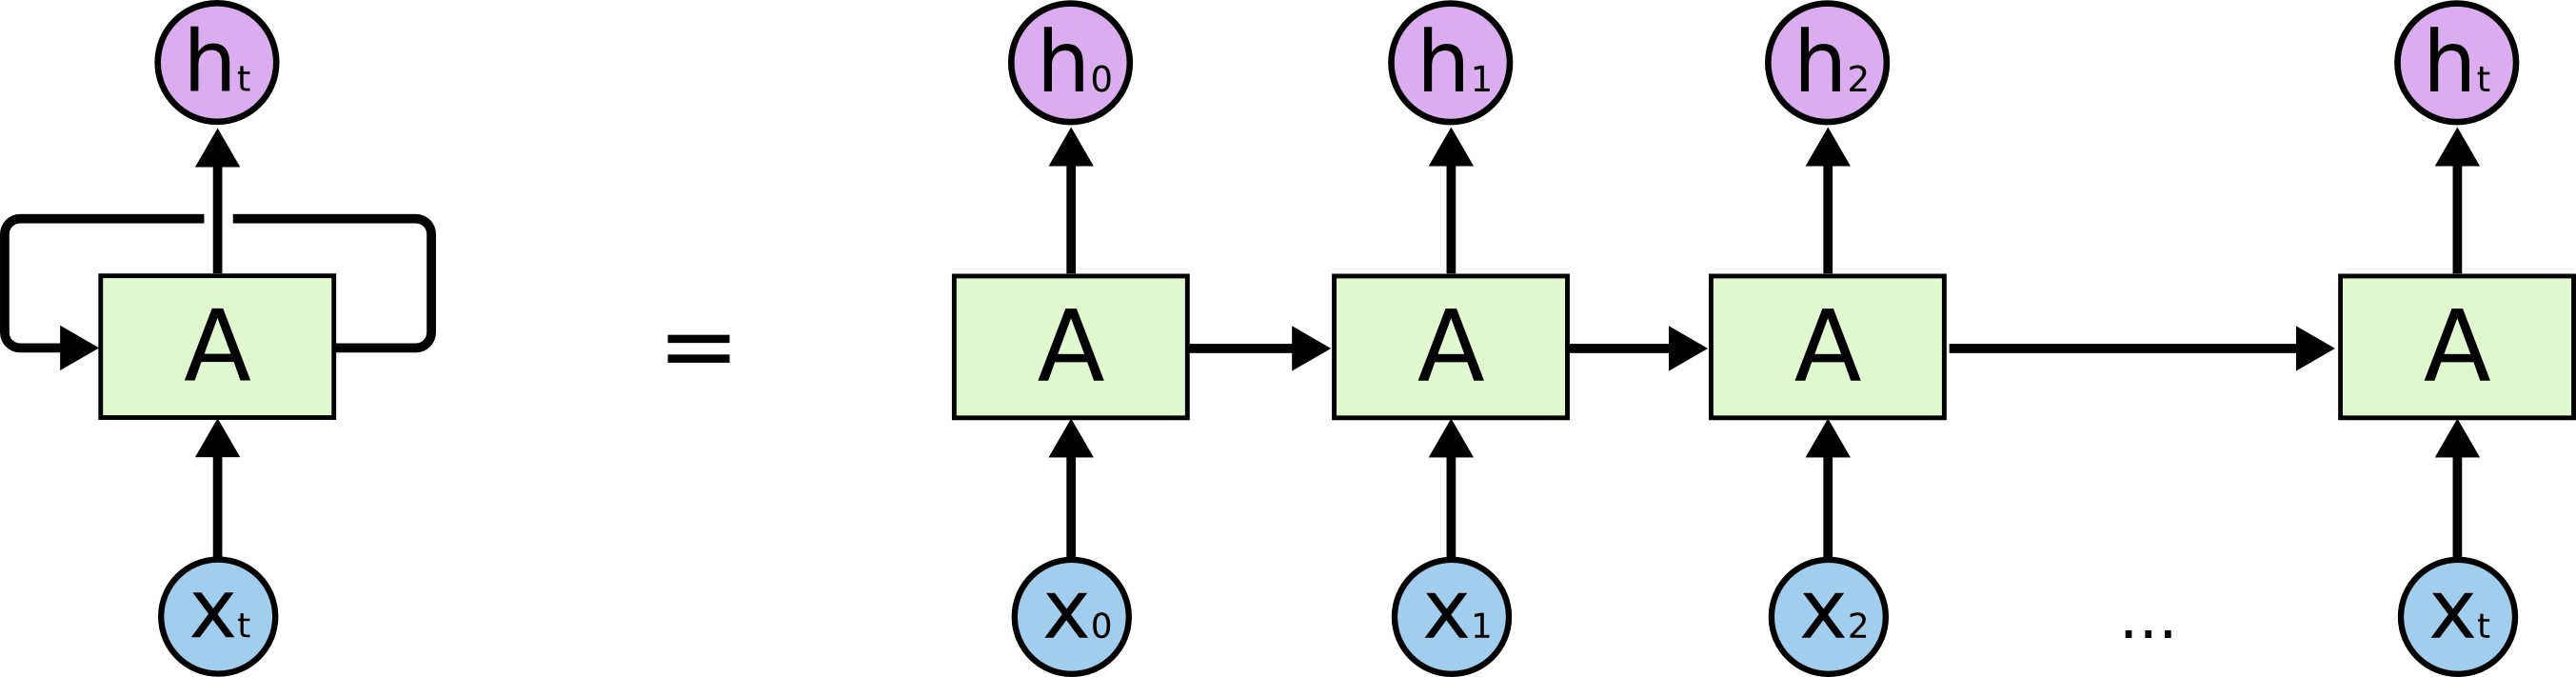
\includegraphics[width=0.8\textwidth]{data/Figures/LSTM/LSTM.png}
    \caption[Unrolled recurrent neural network]{An unrolled recurrent neural network.}\label{fig:Decomposition}
\end{figure}

https://towardsdatascience.com/lstm-networks-a-detailed-explanation-8fae6aefc7f9
\subsubsection{Sigmoid function}
\begin{equation}
    S(x) = \frac{e^x}{e^x+1}
\end{equation}
Since: 
\begin{equation}
    S(x) = \frac{e^x}{e^x+1}
\end{equation}
\subsubsection{Hyperbolic tangent function}
\begin{equation}
    S(x) = \frac{sinh(x)}{cosh(x)} = \frac{e^x-e^{-x}}{e^x+e^{-x}}
\end{equation}